
%matplotlib inline: esto es para que las graficas aparescan a dentro.

\documentclass{article}
%Reporte de computacional
%matplotlib inline: esto es para que las graficas aparescan a dentro.
\usepackage{hyperref}
\usepackage{amsmath}
\usepackage{amsthm}
\usepackage{amssymb}
\usepackage{graphicx}
\usepackage{ifxetex}
\ifxetex
\usepackage{fontspec}
\else
\usepackage[T1]{fontenc}
\usepackage[utf8]{inputec}
\usepackage{lmodern}
\fi



\begin{document}
\title{Sistemas de resortes acoplados}
\author{Ramses Pacheco Ortiz}
\date{ De Febrero Del 2018}
\maketitle  


\section{Introducción}

En esta actividad,tiene como objetivo la modelación de fenómenos físicos, apoyados con Python(jupyter lab).Iniciaremos estudiando la ley de hooke u oscilaciones,un tema antes visto en la materia de mecanica 1 y 2 ,en la cual aplicaremos nuestro conocimiento,para esto nos basaremos en un archivo llamado "coupled springs equations"
de los autores Fay y Graham.
analizaremos cuatro casos en donde cada uno de ellos cuenta con ciertos parametros conocidos como las constantes k de resortes, masas,desplazameintos,longitud natural,etc.


presentaremos el codigo que se utilizo para resolver dicho problema mostrando su error relativo en lo calculado utilizando la biblioteca scipy.integrate.odeint para despues compararlo con la solucion que nos presenta dicho articulo,incluiremos una serie de  graficas generadas por los datos, y para finalizar mostreremos un conclusion general,basados en unas preguntas reflexivas sobre lo aprendido.

\section{Modelo de resortes acoplados}

la sigueinte imagen muestras el sistema de resortes acoplados:

\begin{center}
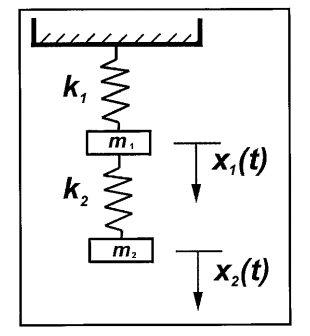
\includegraphics[height=5cm]{sistema.PNG}
\end{center}


Como se puede ver en la imagen el modelo consisite en dos resortes y dos masas,un resorte con una constante$k1$ esta sujetado del techo colgando un masa( $m1$), y en este mismo resorte esta sujetado el segundo resorte con una constante $k2$ tambien colgando un masa($m2$).
 el sistema permite que  descanse en equilibrio, medimos el desplazamiento del centro de masa de cada peso del equilibrio, como una función del tiempo medidas por $x1(t)$ y $x2(t)$, respectivamente.
 
Asumiendo que el sistema se mueve en oscilaciones pequeñas, y debido a la ley de hooke, la fuerza restauradora que presentaron los resortes seran de la forma $k1l1$ y $k2l2$ respectivamente donde $l1$ y $l2$ son las elongaciones o compresiones de los resortes.

realizando un diagrama de fuerzas en el sistema y aplicando la ley de newton podemos destacar estas 2 ecuaciuon siguientes al momento de hacer la sumatoria de fuerzas:

\begin{center}
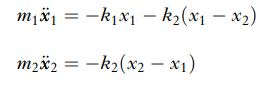
\includegraphics[height=2cm]{ec1.png}
\end{center}

De esta manera obtendremos un par ecuaciones diferenciales de segundo orden, encontrando una ecuación para $x1$ pero que no involucre la variable $x2$ despejando a $x2$ nos queda:

\begin{center}
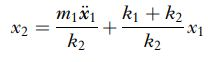
\includegraphics[height=1cm]{ec2.png}
\end{center}

sustituyendo $x2$ en la segunda ecuacion diferencial y simplificando obtenemos:

\begin{center}
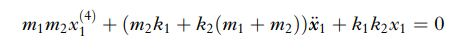
\includegraphics[height=1cm]{ec3.png}
\end{center}

podemos ver que el movimiento de la primera masa ya esta determinada por la ecuacion lineal de cuarto orden, ahora para botener un cuacion que solo involucre la variable $x2$
despejaremos la $x1$ de la segunda ecuacion diferencial:

\begin{center}
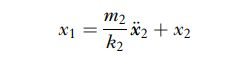
\includegraphics[height=2cm]{ec4.png}
\end{center}

sustituyendo la ecuacion anterior en la primera ecuacion y simplificando nos que da:

\begin{center}
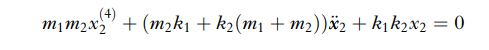
\includegraphics[height=1cm]{ec5.png}
\end{center}

podemos observar que esta ultima ecuacion tiene la misma estructura que la ecuacion para el primer resorte y si consideramos que las masas de los dos resortes vale $1kg$ podemos simplificarla dando nos la siguiente ecuacion:
 
 
\begin{center}
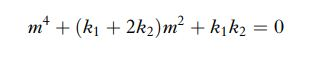
\includegraphics[height=1cm]{ec6.png}
\end{center}

la cual sus racies son:

\begin{center}
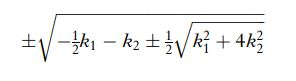
\includegraphics[height=1cm]{ec7.png}
\end{center}

%%%%%%%%%%%%%%%%%%%%%%%%%%%%%%%%%%%%%%%%%%%%%%%%%%%%%%%%%%%
\section{Problemas}
\vspace{0.05cm}
\subsection{Ejemplo 2.1}

Describir el movimiento para las constantes del resorte k1=6 y k2=4 con las condiciones iniciales :

\begin{center}
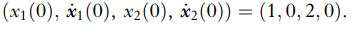
\includegraphics[height=1cm]{ec8.png}
\end{center}

para comenzar primeramente tenemos que establecer el vectorfield que define las ecuaciones del sistema de resorte acoplado, a continuacion se mostrara como se definio el vertorfield:

\begin{center}
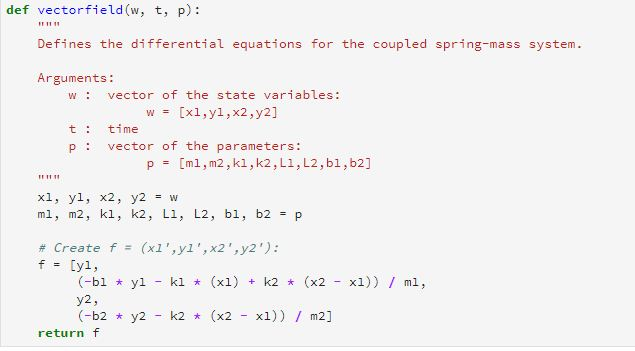
\includegraphics[height=8cm]{cod1.png}
\end{center}

las variables de entrada son w,t,p:
\begin{itemize}
\item w es el vector que contienen los parametros como la  posicion$(xi)$ y la velocidad$(wi)$

\item t es el tiempo
\item p es el vector que contiene varias constantes como la k,logitud(l),masas(m),etc.

\end{itemize}

\vspace{0.5cm}

para proseguir se importan las bibliotecas numpy y spicy con la funcion odeint para poder resolver las ecuaciones diferenciales:

\begin{center}
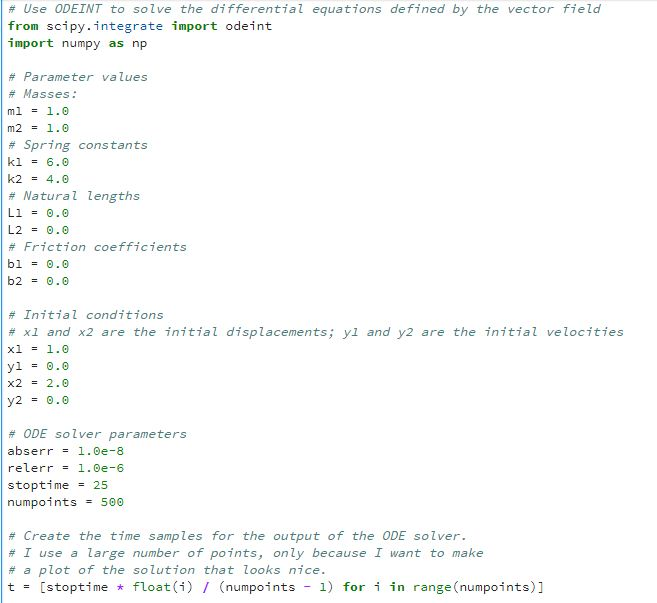
\includegraphics[height=10cm]{cod2.png}
\end{center}

\begin{center}
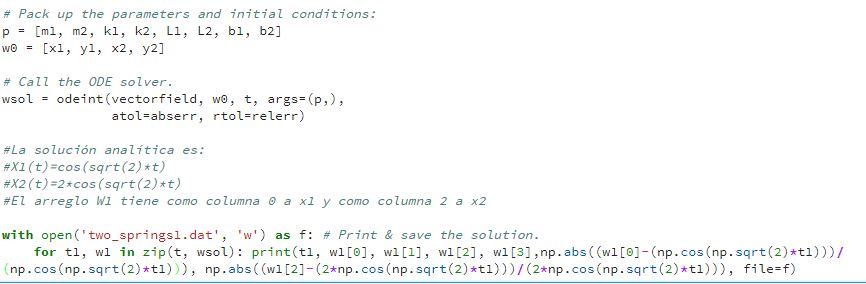
\includegraphics[height=5cm]{cod3.png}
\end{center}

Ya que resolvimos la ecuacion se procedio a graficar los desplazameintos x1 y x2 contra el tiempo, la phase portraits y x1 vs x2:

\begin{center}
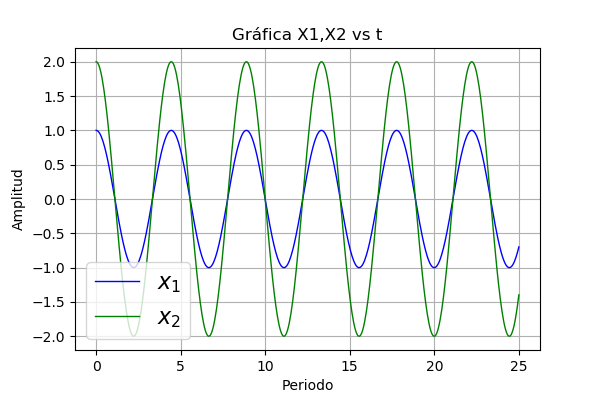
\includegraphics[height=6cm]{resorte2_1.png}
\end{center}

\begin{center}
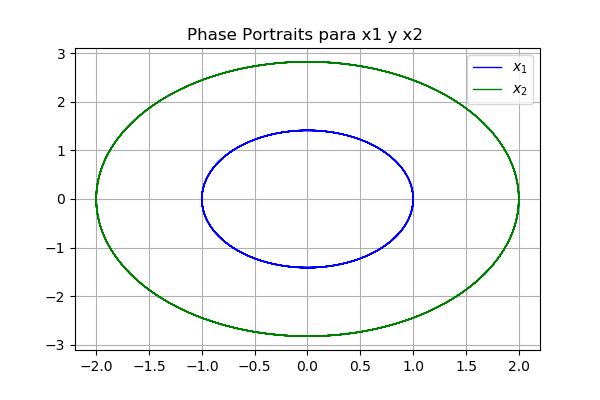
\includegraphics[height=6cm]{resorte2_1_2.png}
\end{center}

\begin{center}
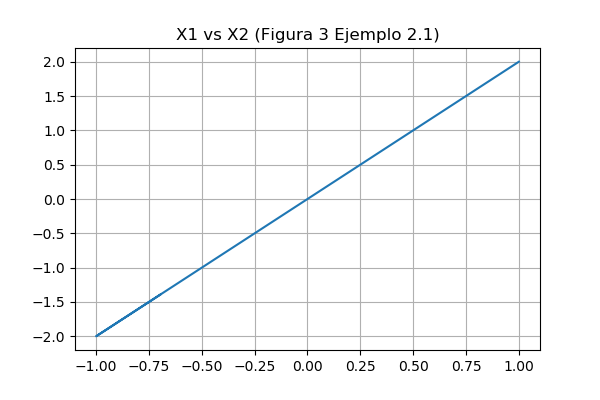
\includegraphics[height=6cm]{resorte2_1_3.png}
\end{center}




la solucion analitica que se obtubo en el articulo esta dada por:

\begin{center}
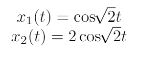
\includegraphics[height=3cm]{ec9.png}
\end{center}

La grafica del error relativo entre la solucion calculada y la que ofrece el articulo es la siguiente:


\begin{center}
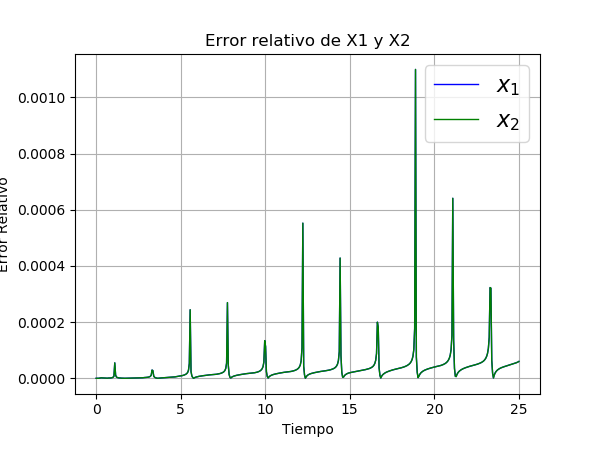
\includegraphics[height=8cm]{ErrorRelativo2_1.png}
\end{center}

%%%%%%%%%%%%%%%%%%%%%%%%%%%%%%%%%%%%%%%%%%%%%%%%%%%%%%%
\subsection{Ejemplo 2.2}

Describir el movimiento para las constantes del resorte k1=6 y k2=4 con las condiciones iniciales :

\begin{center}
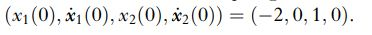
\includegraphics[height=1cm]{ec10.png}
\end{center}

Acontinuacion se muestra el cambio de codigo que se tubo que hacer,recuerde que el vectorfield simepre se realiza en todos los ejemplos:

\begin{center}
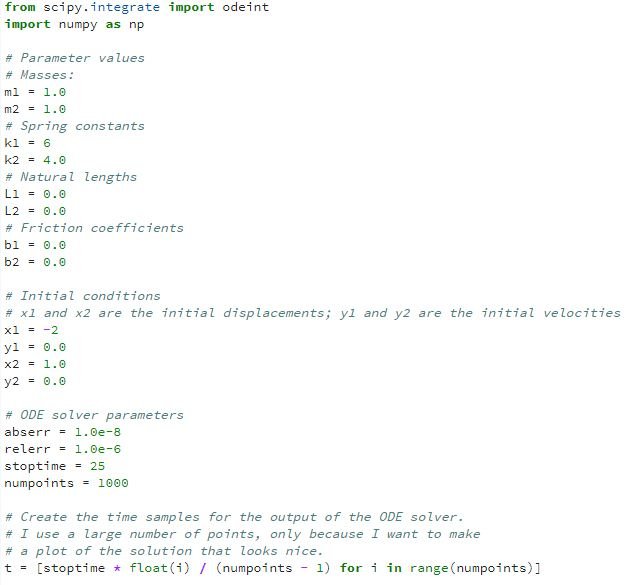
\includegraphics[height=9cm]{cod4.png}
\end{center}

\begin{center}
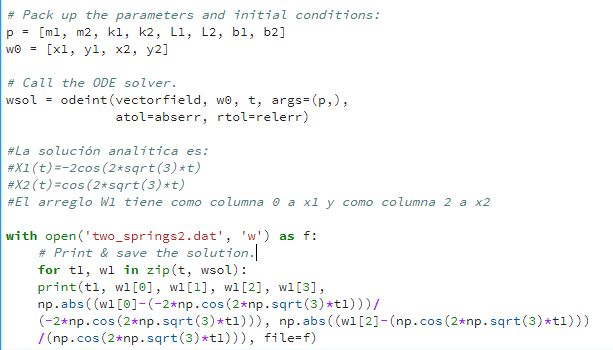
\includegraphics[height=9cm]{cod4_1.png}
\end{center}

\vspace{0.5cm}

Las graficas resultantes son las siguientes:

\begin{center}
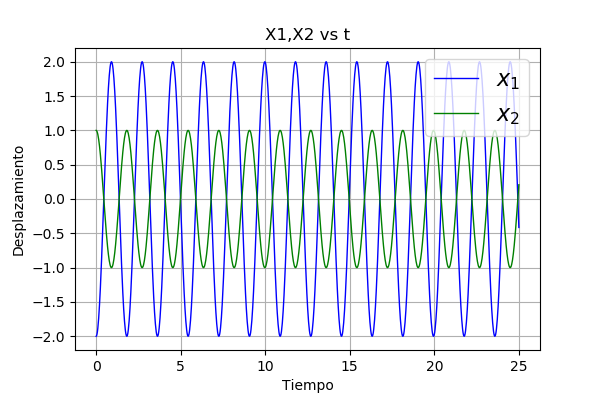
\includegraphics[height=6cm]{resortes2_2_1.png}
\end{center}

\begin{center}
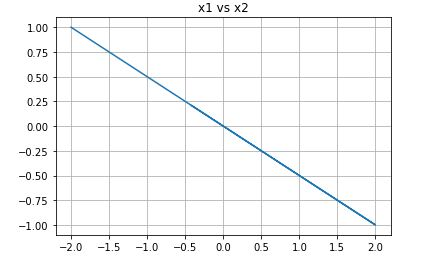
\includegraphics[height=6cm]{resortes2_2_2.png}
\end{center}

La solucion analitica esta dada por:

\begin{center}
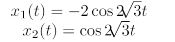
\includegraphics[height=1cm]{ec11.png}
\end{center}


La grafica del error relativo de la solicion calculcalada y la que ofrece el articulo es la siguiente:

\begin{center}
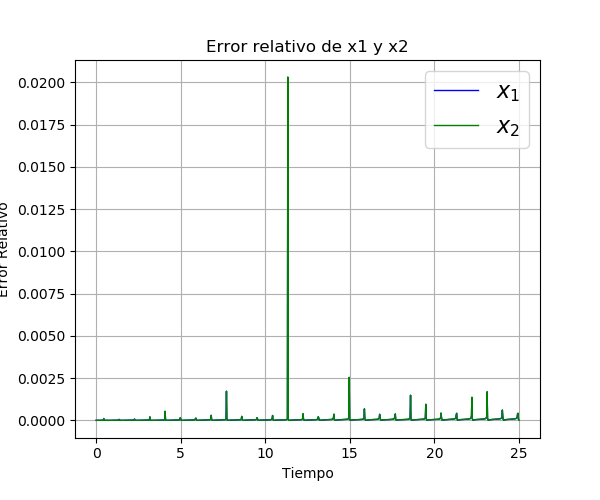
\includegraphics[height=8cm]{ErrorRelativo2_2.png}
\end{center}

%%%%%%%%%%%%%%%%%%%%%%%%%%%%%%%%%%%%%%%%%%%%%%%%%%%

\subsection{Ejemplo 2.3}

Describir el movimiento para las constantes del resorte k1=0.4 y k2=1.808 con las condiciones iniciales :

\begin{center}
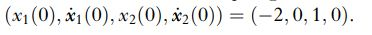
\includegraphics[height=1cm]{ec10.png}
\end{center}

En este ejemplo y en el siguiente no se mostrara el error relativo debido al articulo ya que no muestra la solucion analitica. 


Acontinuacion se muestra el codigo que se modifico:

\begin{center}
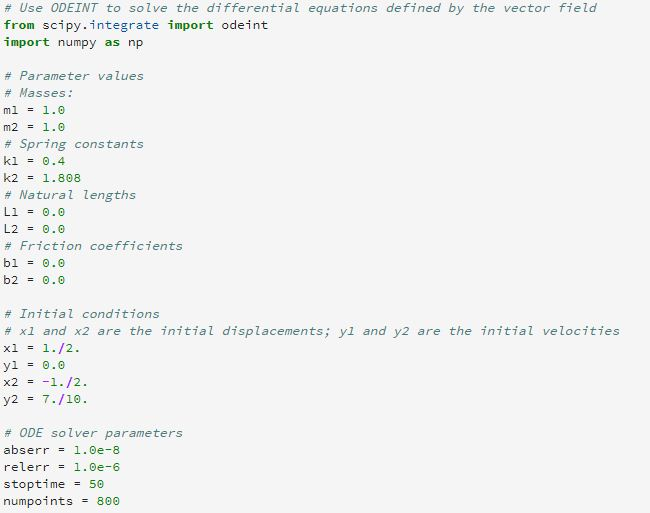
\includegraphics[height=12cm]{cod5.png}
\end{center}

\begin{center}
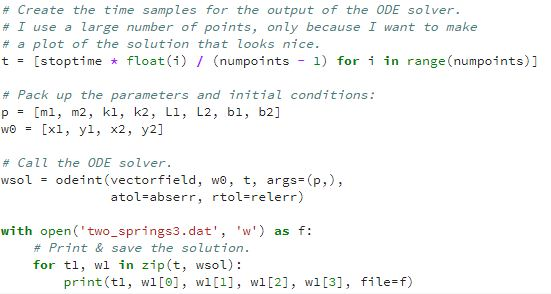
\includegraphics[height=9cm]{cod5_1.png}
\end{center}

Las graficas que se llevaron acabo en este problema son las siguientes:

\begin{center}
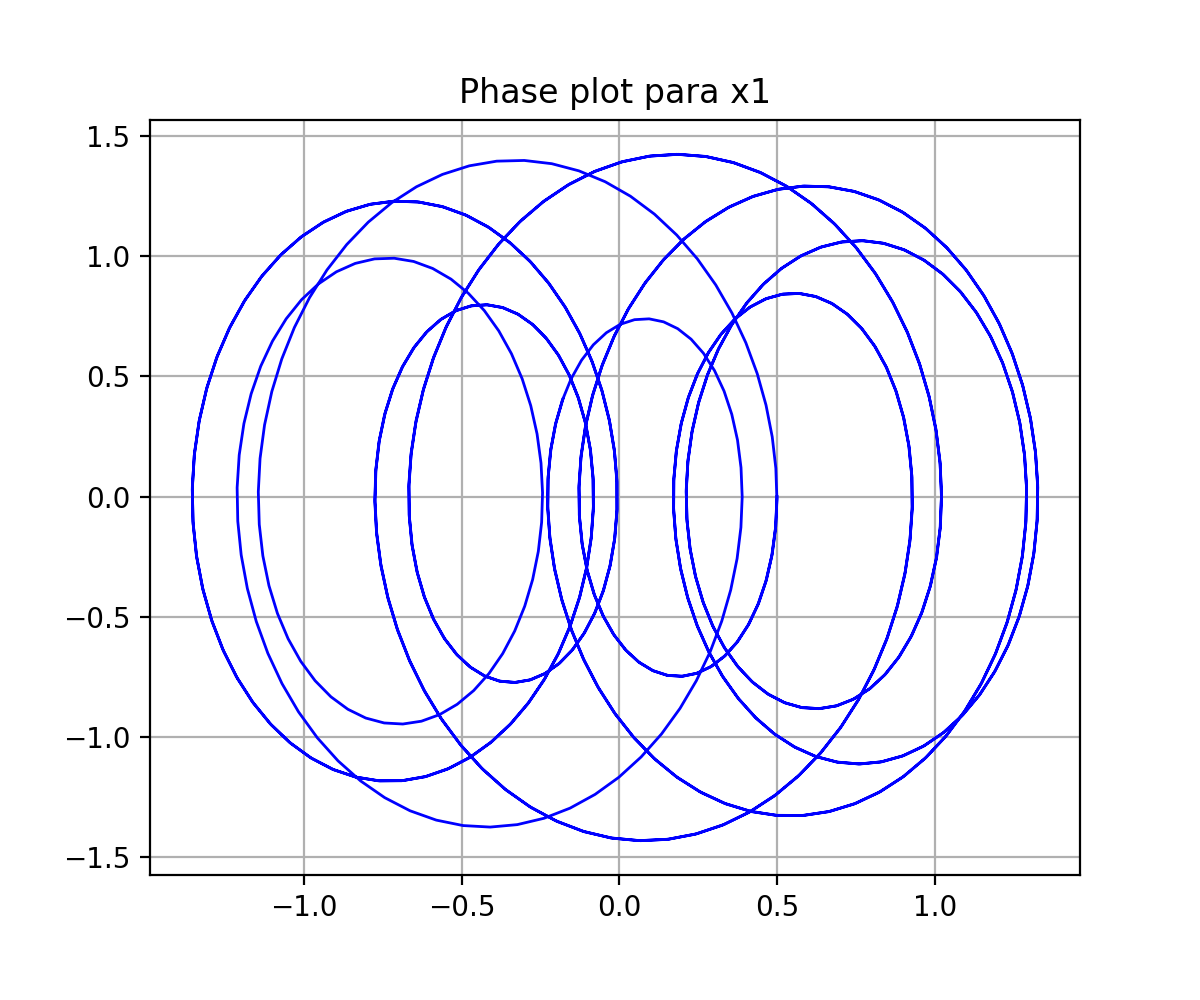
\includegraphics[height=6cm]{resortes2_3_1.png}
\end{center}

\begin{center}
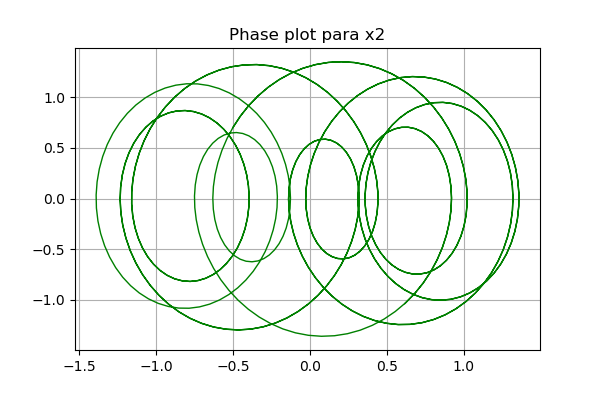
\includegraphics[height=6cm]{resortes2_3_2.png}
\end{center}


\begin{center}
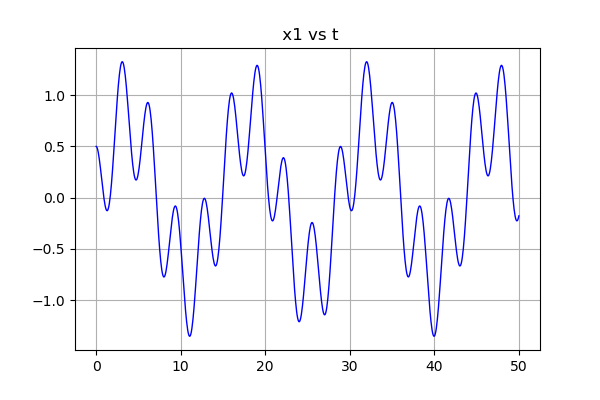
\includegraphics[height=6cm]{resortes2_3_3.png}
\end{center}

\begin{center}
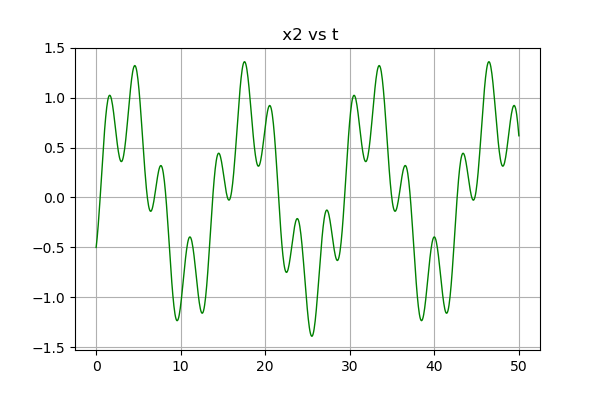
\includegraphics[height=6cm]{resortes2_3_4.png}
\end{center}

\begin{center}
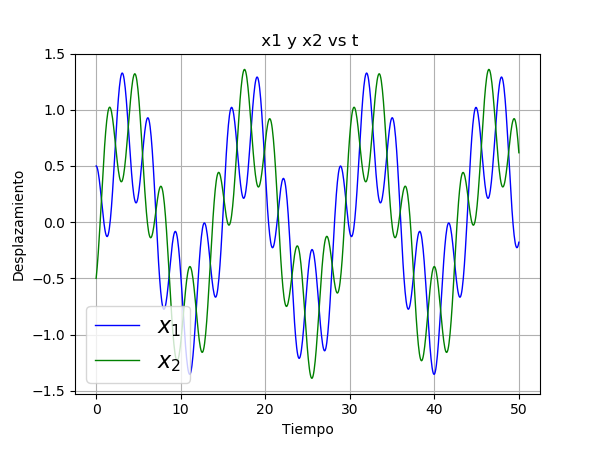
\includegraphics[height=6cm]{resortes2_3_5.png}
\end{center}

\begin{center}
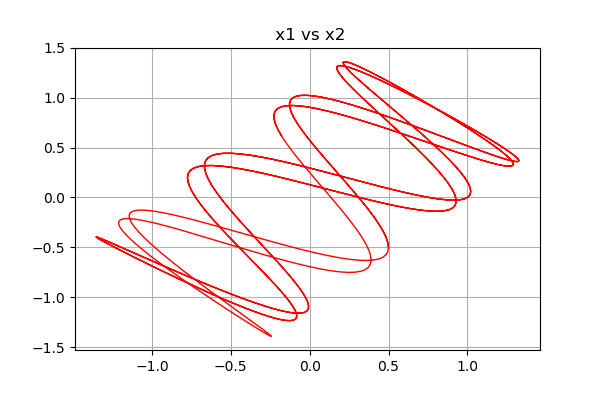
\includegraphics[height=6cm]{resortes2_3_6.png}
\end{center}

%%%%%%%%%%%%%%%%%%%%%%%%%%%%%%%%%%%%%%%%%%%%%%%%%%%%
\subsection{Ejemplo 2.4}

Describir el movimiento para las constantes del resorte $k1=0.4$ y $k2=1.808$ asumiendo que $m1=m2=1$, coeficientes de amortiguameinto $b1=0.1$ y $b2=0.2$ con las condiciones iniciales :

\begin{center}
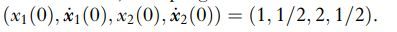
\includegraphics[height=1cm]{ec13.png}
\end{center}

La diferencia que observaran en el sigueinte codigo es que ahora se tomaron encuenta los coeficientes de amortiguamiento

\begin{center}
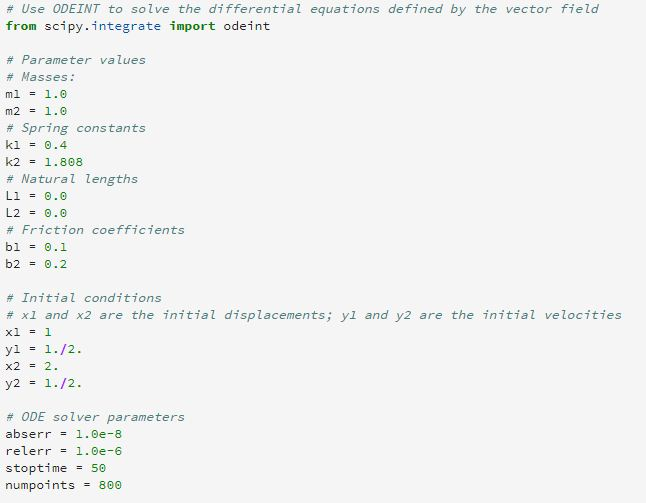
\includegraphics[height=12cm]{cod6.png}
\end{center}

\begin{center}
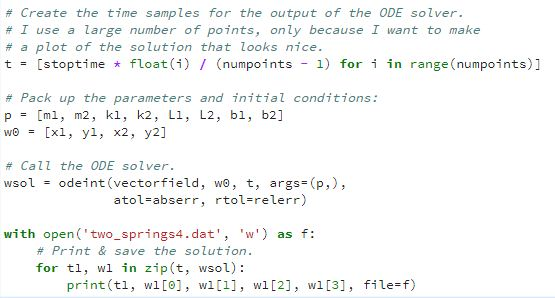
\includegraphics[height=9cm]{cod6_1.png}
\end{center}

Acontinuacion se motraran las graficas que se llevaron a cabo en este ejemplo:
\begin{center}
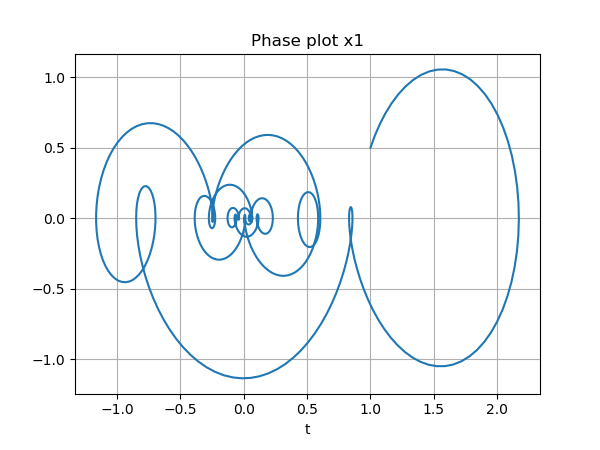
\includegraphics[height=6cm]{resortes2_4_1.png}
\end{center}

\begin{center}
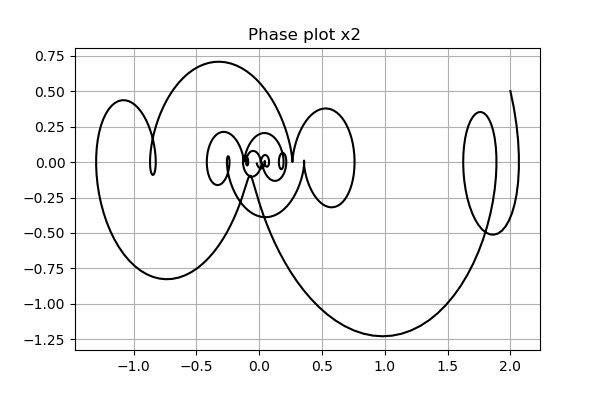
\includegraphics[height=6cm]{resortes2_4_2.png}
\end{center}


\begin{center}
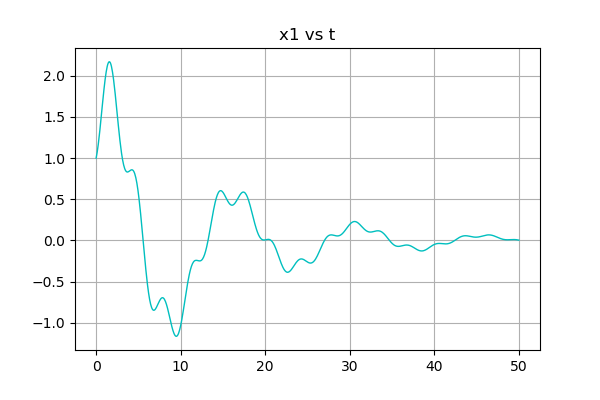
\includegraphics[height=6cm]{resortes2_4_3.png}
\end{center}

\begin{center}
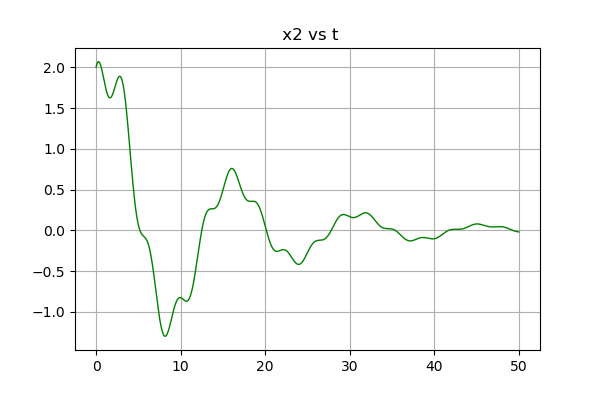
\includegraphics[height=6cm]{resortes2_4_4.png}
\end{center}

\begin{center}
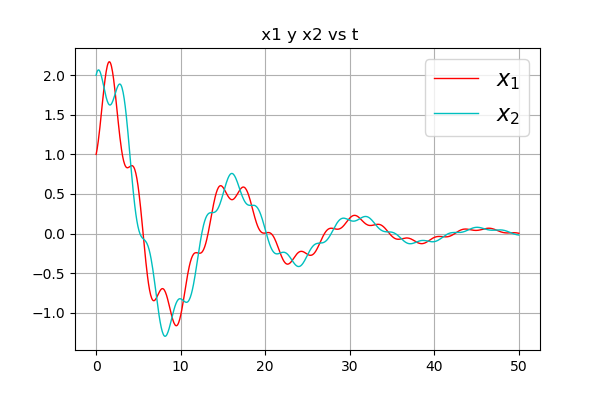
\includegraphics[height=6cm]{resortes2_4_5.png}
\end{center}

\begin{center}
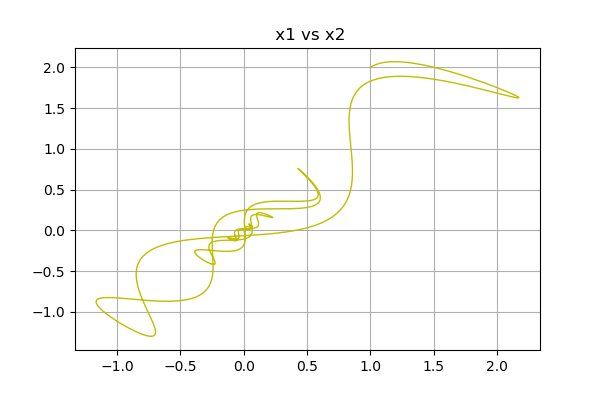
\includegraphics[height=6cm]{resortes2_4_6.png}
\end{center}


\section{Conclusion}

Esta actividad se trabajo con modelados fisicos ,fue un acercamiento a lo que considero un trabajo de un fisico o mas bien aprender a realizar modelados fisicos con ayuda de herramientas computacionales para resolver ecuacion diferenciales que representen dicho modelo ya que es algo que el fisico tiene que hacer dia a dia.

Unas de las observaciones que se puede resalatar al realizar esta practica, son las graficas, como observamos mientras teniamos mas parametros las grafica se fueron haciendo un poco mas "feas" o no tan lineales como las del ejemplo 1 y 2.


\section{Apéndice}

\textbf{¿En general te pareció interesante esta actividad de modelación matemática?}
 Me gusto mucho ya que me sirvo repasar esos tipos de probemlas sobre la ley de hooke y la materia de ecuaciones diferenciales

\vspace{0.3cm}

\textbf{¿Qué te gustó mas? ¿Qué no te gustó?}


Me gusto mucho el tema escogido ya que es un tema que me gusta mucho ya que es algo que vemos en la vida diaria o que podemos aplicarla.
\vspace{0.3cm}


\textbf{La cantidad de material te pareció ¿bien?, ¿suficiente?, ¿demasiado?}

La cantidad de material me paracio algo bien ya que se nos dio la oportunidad de observar diferentes tipos de graficas

\vspace{0.3cm}
\textbf{¿Cuál es tu primera impresión de Jupyter Lab?}


La verdad me senti muy como con la plataforma muy similar al jupyter notebook.

\vspace{0.3cm}

\textbf{Respecto al uso de funciones de SciPy, ¿ya habías visto integración numérica en tus cursos anteriores? ¿Cuál es tu experiencia?.}

Si, ya habiamos visto integracion numerica en la materia de analisis numerico,lvdd esta muy padre pero no recurdo muy bien mis programas.

\vspace{0.3cm}

\textbf{El tema de sistema de masas acopladas con resortes, ¿ya lo habías resuelto en tu curso de Mecánica 2? } 

La verdad no lo recuerdo, pero si recuerdo aver visto la ley de hooke y oscilaciones.


\vspace{0.3cm}
¿Qué le quitarías o agregarías a esta actividad para hacerla más interesante y divertida? 

Esta muy bien organizada.




\vspace{0.3cm}












\end{document}
